% https://stackoverflow.com/a/4170985/5270873

\documentclass{standalone}
\usepackage{tikz}
\usetikzlibrary{decorations.pathmorphing}


\begin{document}

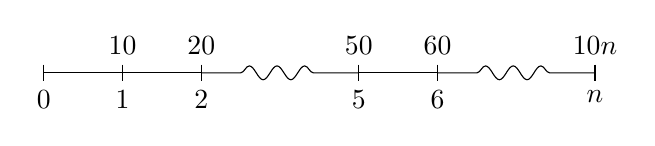
\begin{tikzpicture}
	%draw horizontal line
	\draw (0,0) -- (2,0);
	\draw[decorate,decoration={snake,pre length=5mm, post length=5mm}] (2,0) -- (4,0);
	\draw (4,0) -- (5,0);
	\draw[decorate,decoration={snake,pre length=5mm, post length=5mm}] (5,0) -- (7,0);
	
	%draw vertical lines
	\foreach \x in {0,1,2,4,5,7}
	\draw (\x cm,3pt) -- (\x cm,-3pt);
	
	%draw nodes
	\draw (0,0) node[below=3pt] {$ 0 $} node[above=3pt] {$   $};
	\draw (1,0) node[below=3pt] {$ 1 $} node[above=3pt] {$ 10 $};
	\draw (2,0) node[below=3pt] {$ 2 $} node[above=3pt] {$ 20 $};
	\draw (3,0) node[below=3pt] {$  $} node[above=3pt] {$  $};
	\draw (4,0) node[below=3pt] {$ 5 $} node[above=3pt] {$ 50 $};
	\draw (5,0) node[below=3pt] {$ 6 $} node[above=3pt] {$ 60 $};
	\draw (6,0) node[below=3pt] {$  $} node[above=3pt] {$  $};
	\draw (7,0) node[below=3pt] {$ n $} node[above=3pt] {$ 10n $};
\end{tikzpicture}

\end{document}